\documentclass{beamer}
\usepackage{graphicx}
\usepackage{listings}
\usepackage{beamerthemesplit}
\usetheme{pureminimalistic}

\title{Moogle!}
\author{William Barrios}
\date{23 de julio de 2023}



\begin{document}

\begin{titlepage}

   \begin{center}
    
\includegraphics[scale=0.25]{Imagenes/moogle.png}
   \end{center}

\end{titlepage}

\centering

\section{Qué es Moogle!}

\begin{frame}{Qué es Moogle!}
    Moogle! es una aplicación totalmente original cuyo propósito es buscar inteligentemente un texto en un conjunto de documentos. Es una aplicación web, desarrollada con tecnología .NET Core 6.0, específicamente usando Blazor como framework web para la interfaz gráfica, y en el lenguaje CSharp.
\end{frame}


\section{Características}

\subsection{Características}

\begin{frame}{Características}

    \begin{itemize}
        \item<1-> Búsquedas rápidas. Ofreciendo resultados al momento.(En proceso)
        \item<2-> Determina los términos más relevantes y prioriza los documentos que los contienen.
        \item<3-> Muestra los resultados más importantes primero.
        \item<4-> Muestra fragmentos de los documentos.
        \item<5-> Ofrece sugerencias ante palabras mal escritas o que dan pocos resultados.
        \item<6-> Operadores para controlar el comportamiento de la búsqueda.
    \end{itemize}

\end{frame}

\subsection{Ejemplos}

\begin{frame}{Operadores}
   Buscas una frase en concreto?\\
    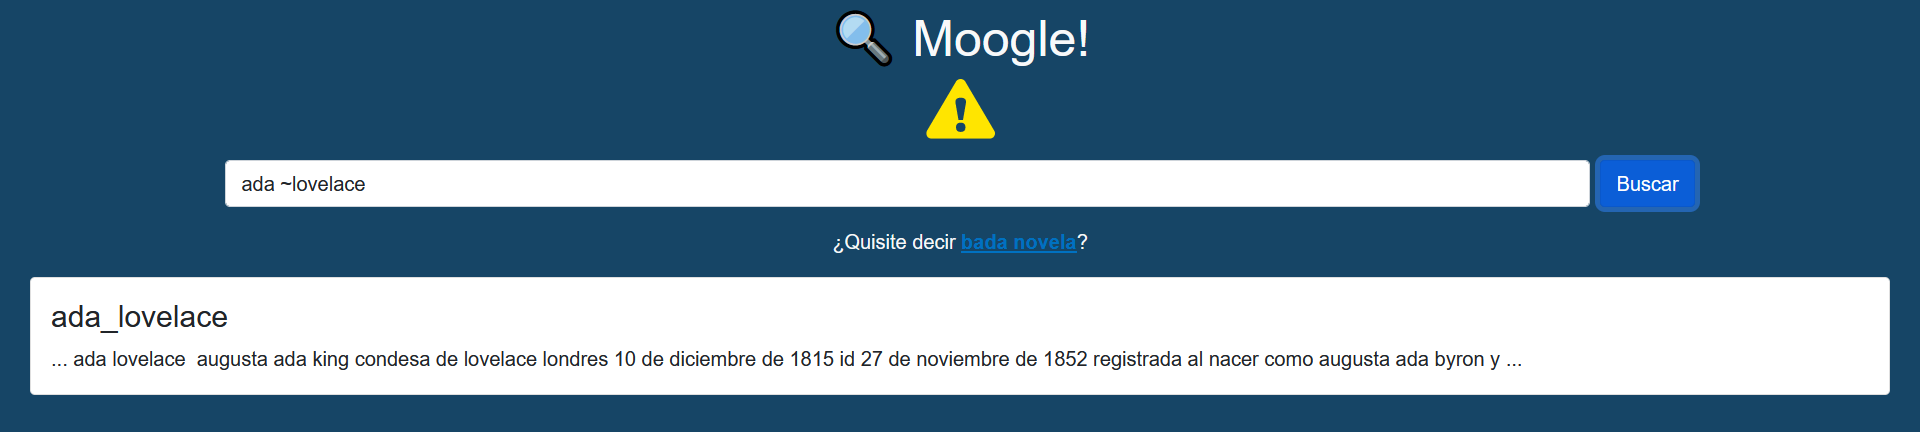
\includegraphics[scale=0.2]{Imagenes/operator_near.png}
\end{frame}

\begin{frame}{Operadores}
    Entendemos lo que quisiste decir\\
    \bigskip
    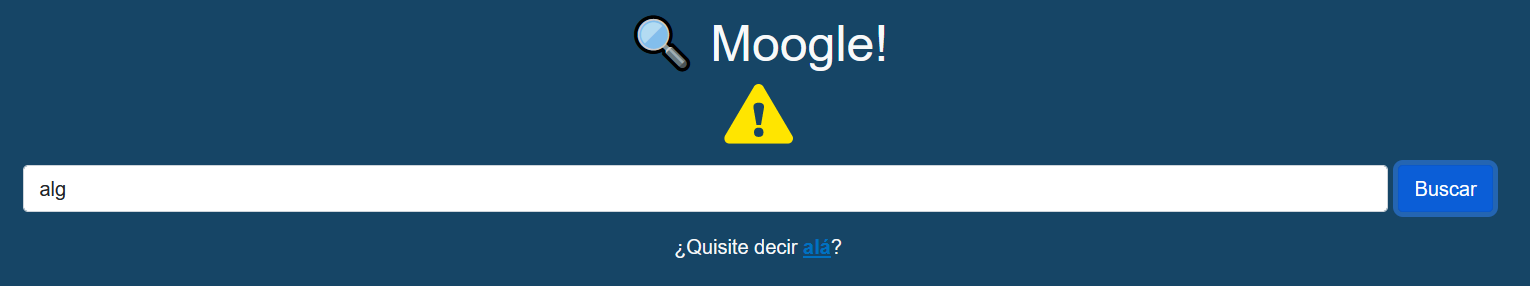
\includegraphics[scale=0.2]{Imagenes/suggestion.png}
\end{frame}

\begin{frame}{Operadores}
    Buscas una palabra con cierta relevancia?\\
    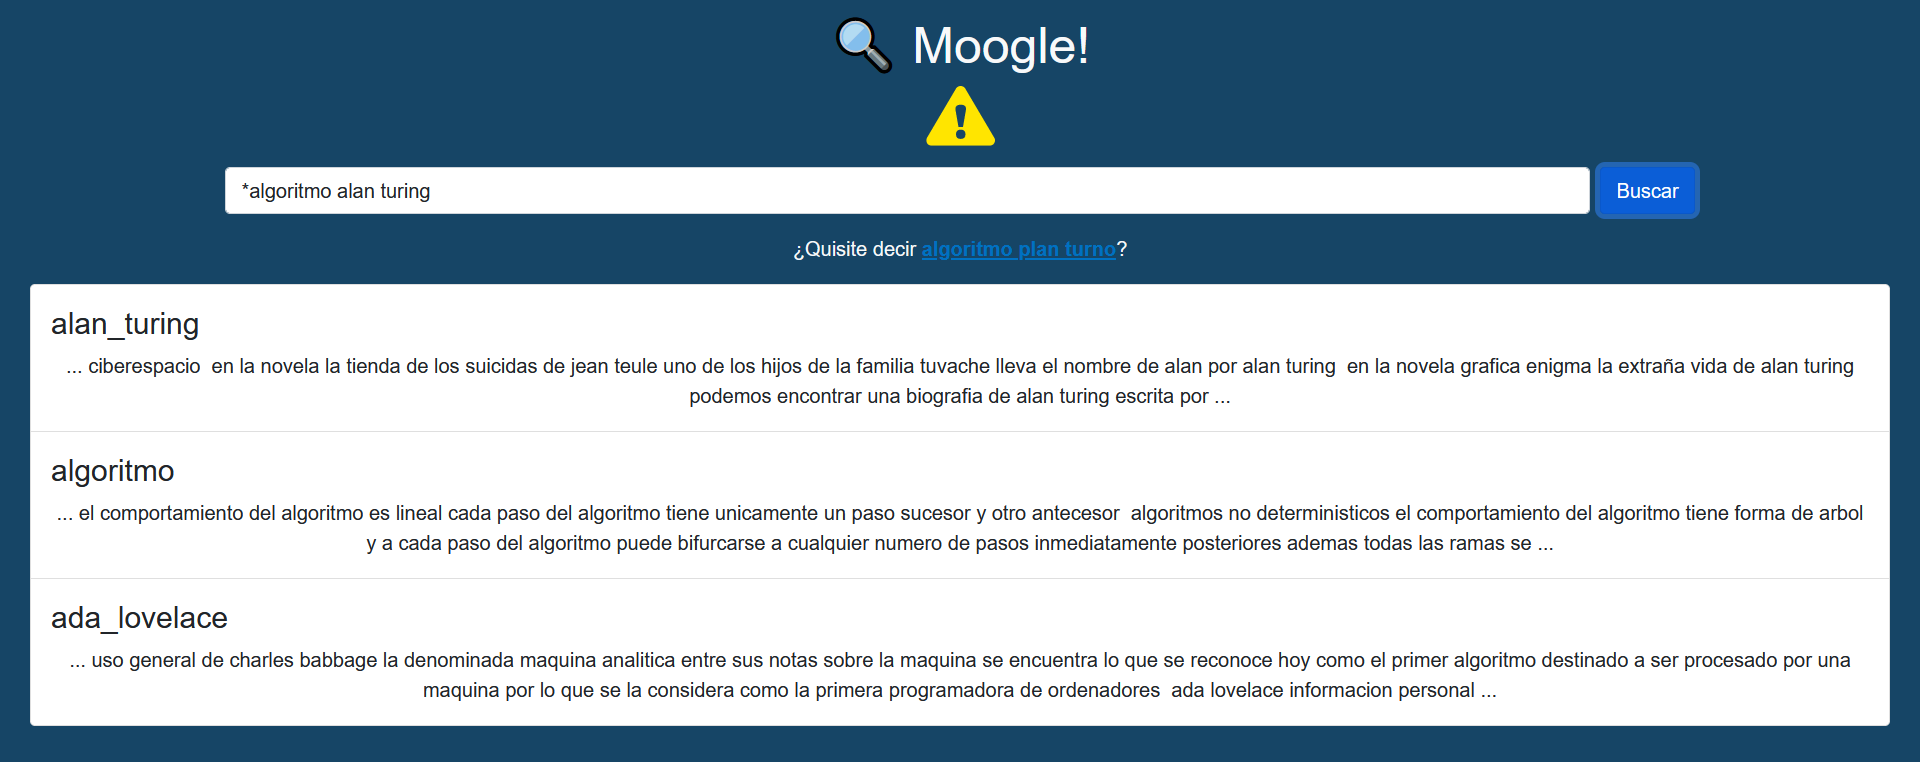
\includegraphics[scale=0.2]{Imagenes/operator_importance.png}
\end{frame}

\begin{frame}{Operadores}
    Buscas algo en concreto pero hay contenido que no te interesa?\\
    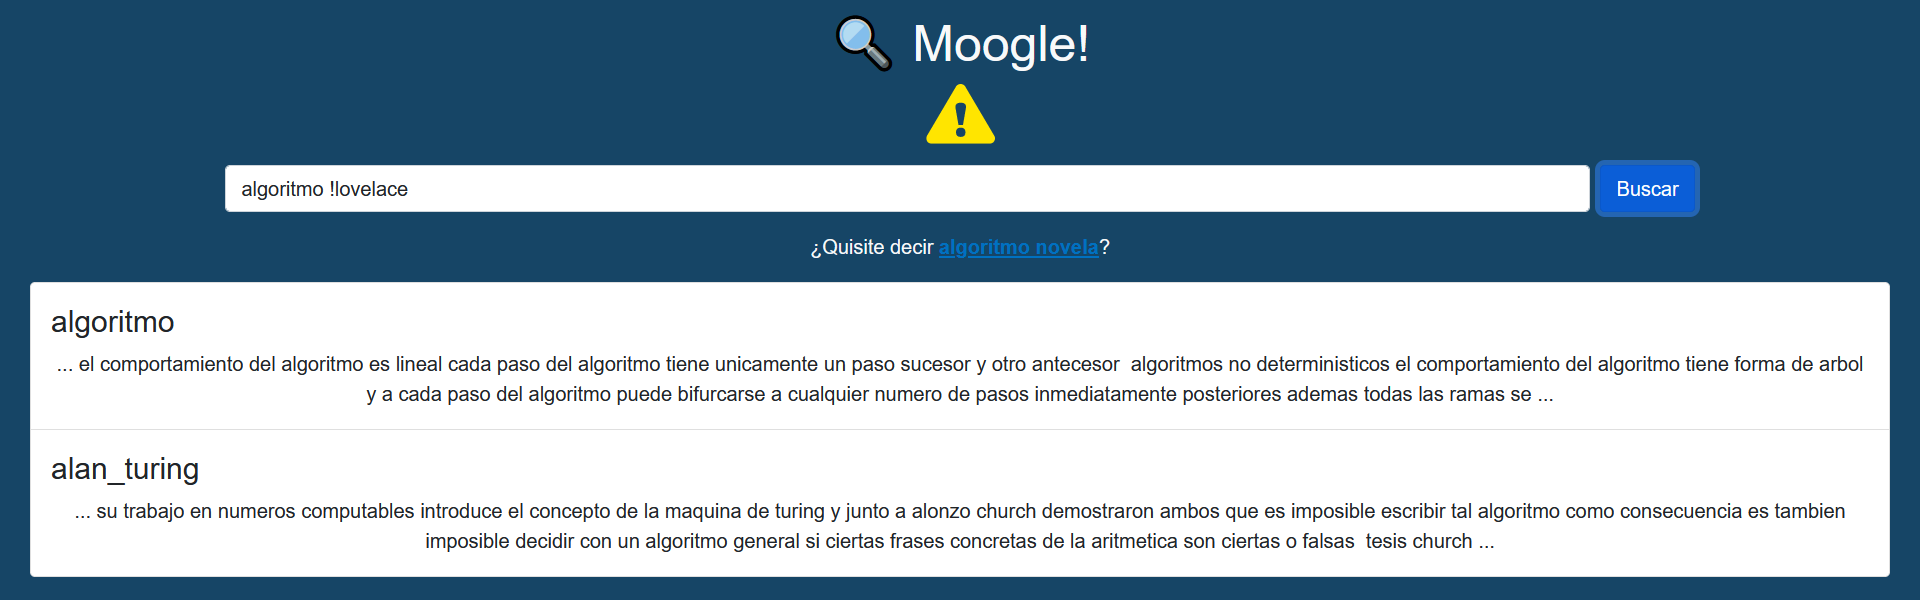
\includegraphics[scale=0.2]{Imagenes/operator_none.png}
\end{frame}

\begin{frame}{Operadores}
    Buscas algo en concreto?\\
    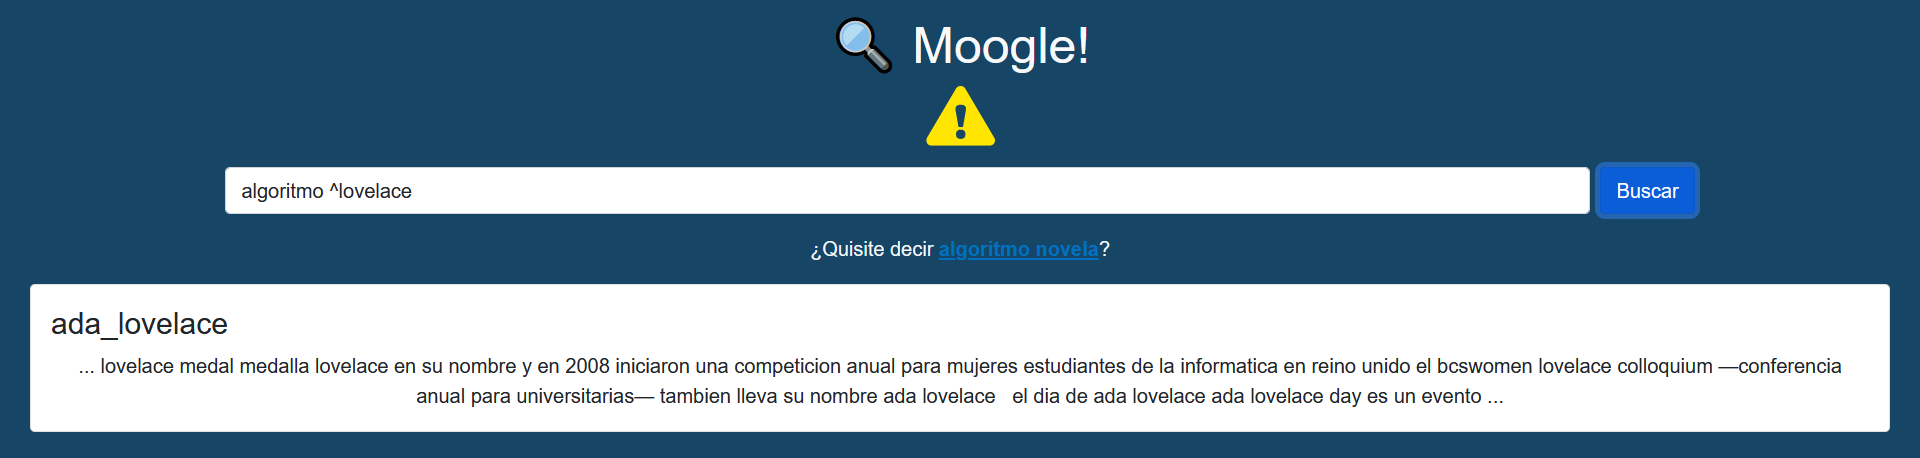
\includegraphics[scale=0.2]{Imagenes/operator_appear.png}
\end{frame}

\begin{frame}{}
        Y eso seria todo, disfruten usando moogle
\end{frame}

\end{document}